\documentclass{article}
\renewcommand{\thesubsection}{\thesection.\alph{subsection}}

\addtolength{\oddsidemargin}{-.875in}
\addtolength{\evensidemargin}{-.875in}
\addtolength{\textwidth}{1.75in}
\addtolength{\topmargin}{-.875in}
\addtolength{\textheight}{1.75in}
	
\usepackage{bm}
\usepackage{amsmath}
\usepackage{amssymb}
\usepackage{tikz}
\usetikzlibrary{automata,positioning}
\usepackage{url}
\usepackage{float}
\usepackage{setspace}


\begin{document}
%\raggedright
\doublespacing

\title{Week 1 Journal}
\author{Rodger Byrd}
\maketitle

%summary info here

\section{Course Goals}
My primary goal for this course are to determine whether I want to pusue a Doctor of Philosophy degree. My other goals include determining whether I'm interested in reasearch, and I would particularly like to learn how to analyze data and show statistical relevance to support a hypothesis. I'd like to learn what kind of tests you can perform on the data to support your hypothesis. I'm studying Computer Science and this will be the last class I take for my master's degree. I completed my undergraduate studies in Electrical Engineering, but I've mostly worked in the fields of software development and cyber security.
\begin{figure}[H]
  \centerline{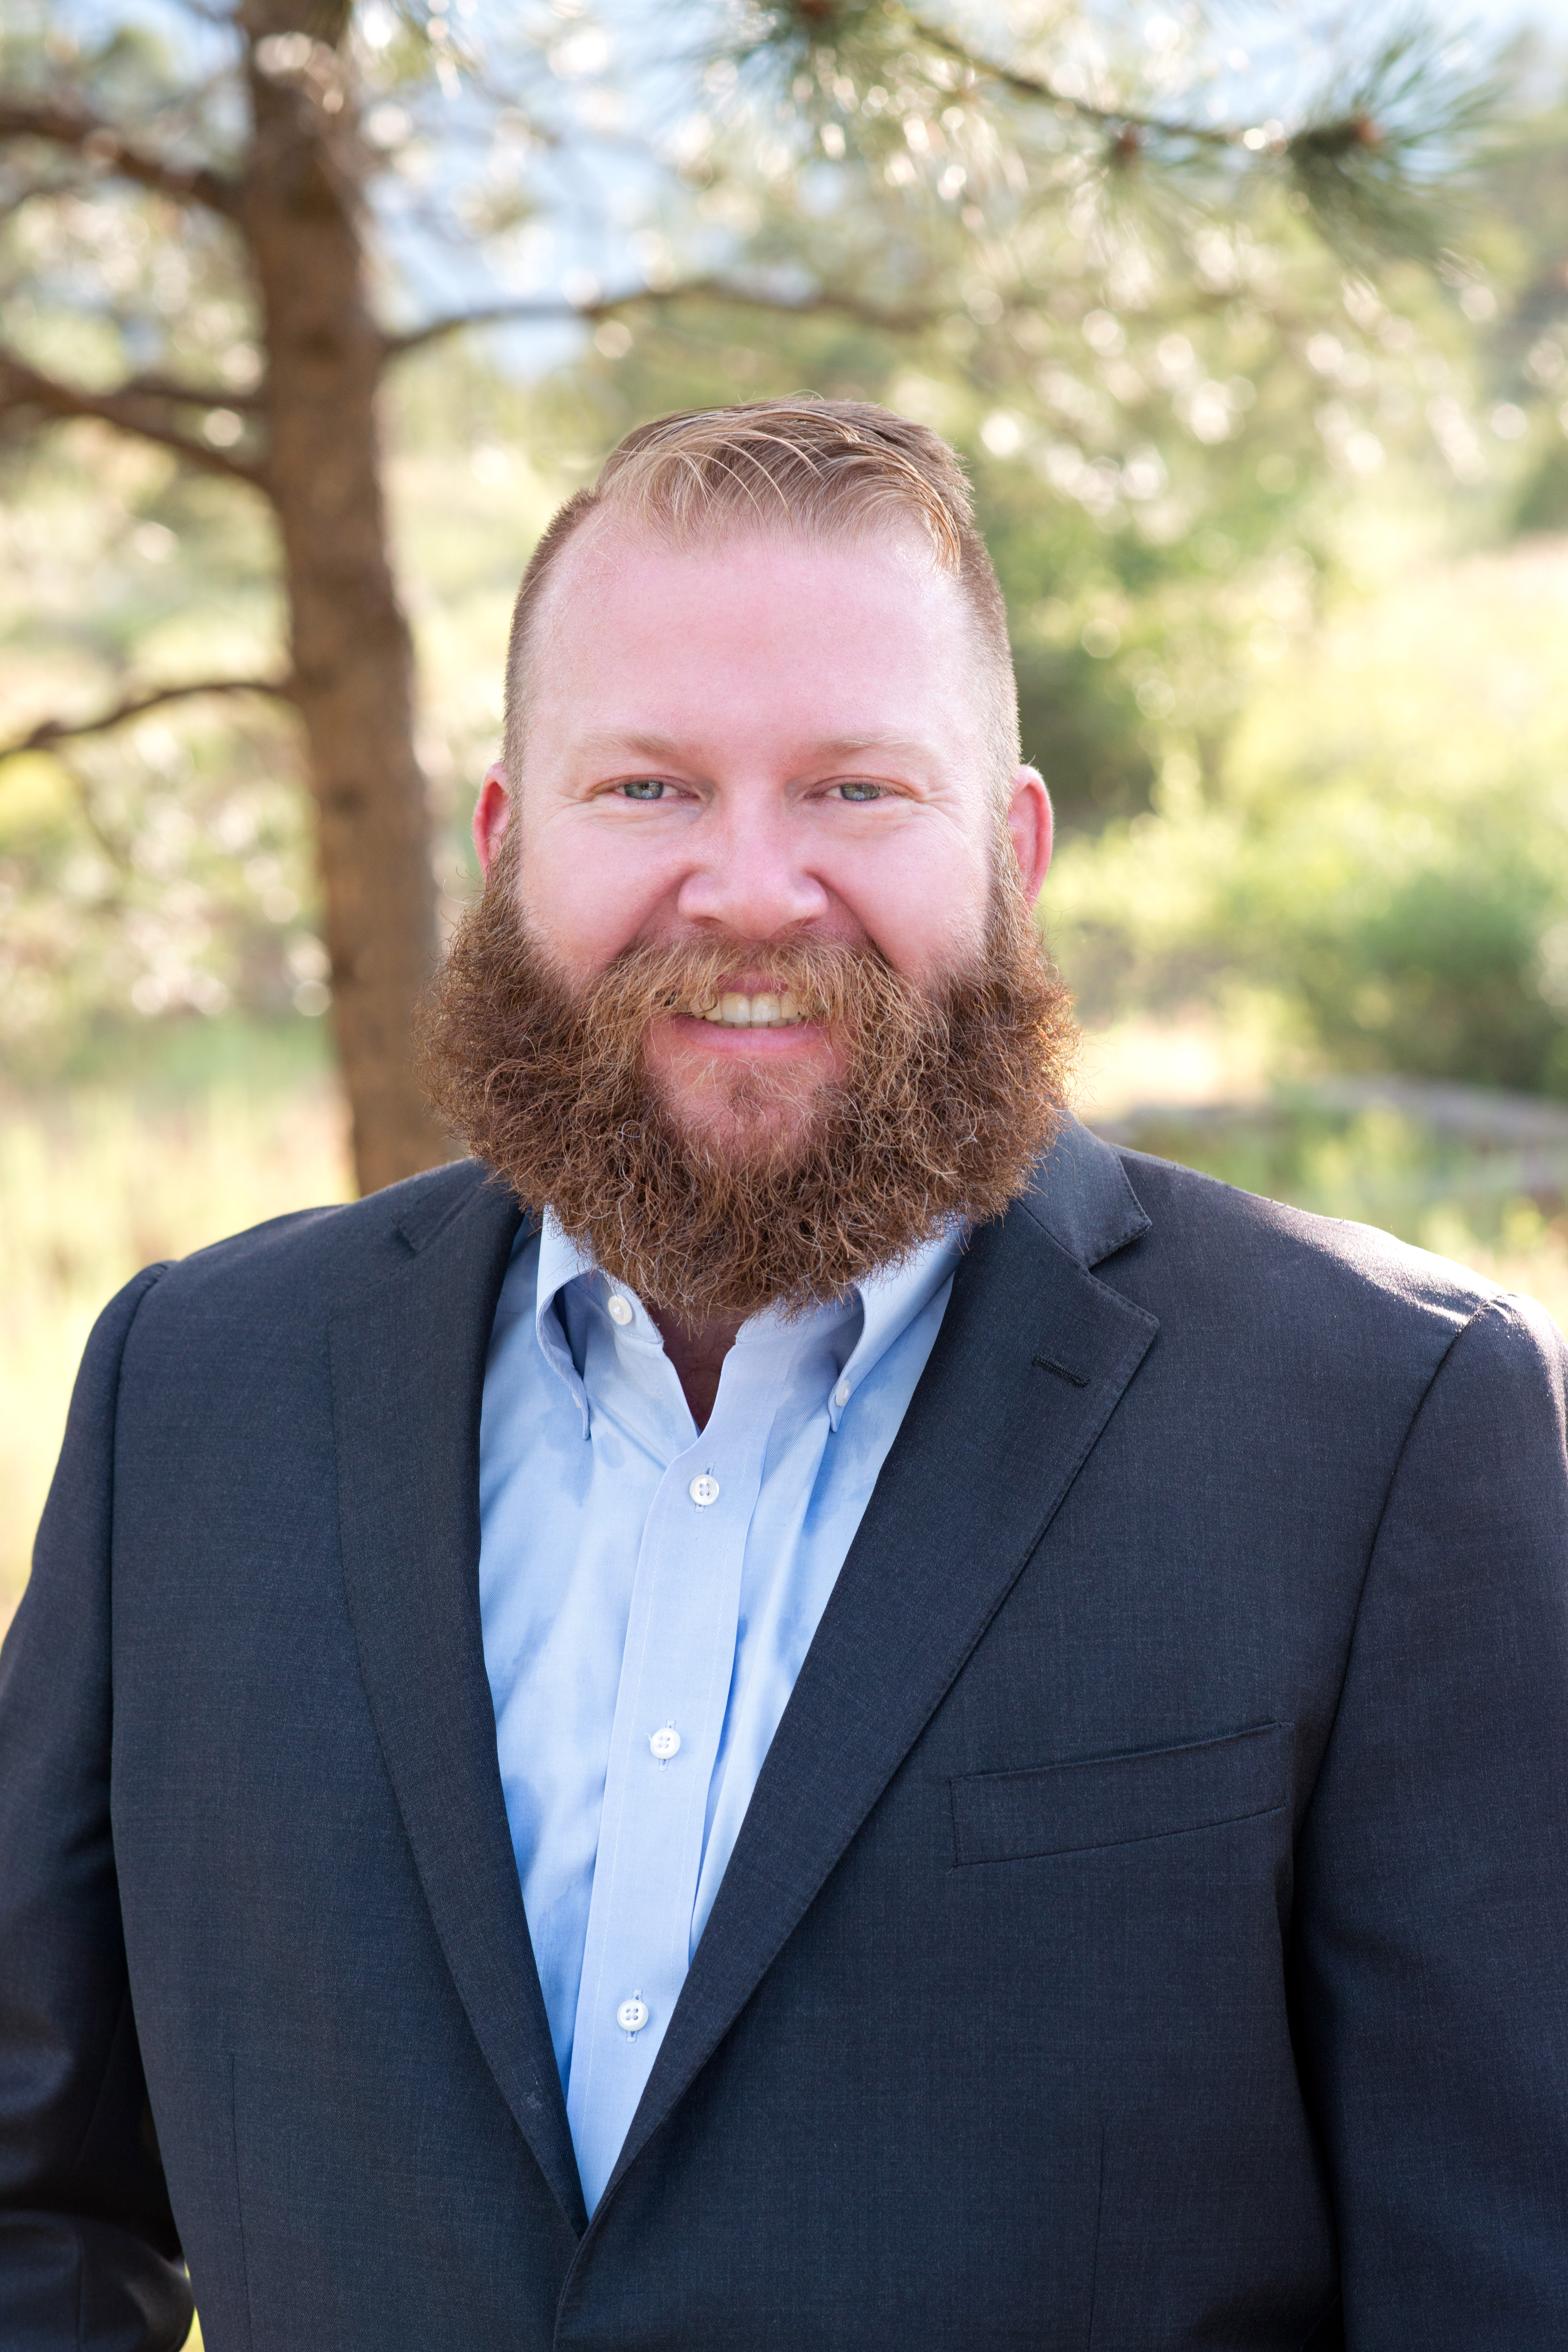
\includegraphics[width=50mm]{headshot.jpg}}
  \caption{Rodger Byrd Headshot}
  \label{fig:HS}
\end{figure} 
I work full time for an engineering consulting firm in the field of cybersecurity. My main motivation for graduate school was to become credentialed in the specific field that I've been working in since I completed my Bachelor's Degree, and possibly open up more career options. I have two young children and with career my available free time is constrained, so the decision to pursure more education after I complete my Master's Degree is a difficult one. I'm hoping this course will help to inform that decision. I've included a picture of myself below in figure \ref{fig:HS}.

\section{Git Repository}
The files for this latex document are in the github repository located at \path{https://github.com/rodger79/CS6000}. I used Texmaker to build the pdf from the latex files.

Summarize Learing here: problem/struggles you had and how you overcame them.

\section{Research}


\begin{thebibliography}{9}
\bibitem{git} 
Project github, \\\path{https://github.com/rodger79/CS6000}
\bibitem{jflap} 
JFLAP, \\\path{http://www.jflap.org/getjflap.html}
\end{thebibliography}

\end{document}